%!TEX root = ../MasterThesis.tex

\section{\gls{RDF} vocabularies and Web Ontologies for \gls{E-commerce}}
\label{sec:choose_data_schema}

As a major objective of the \gls{E-commerce} fraud investigation system is to collect the various transactional information from online merchants, \gls{PSP}s and issuers, combine and link them together, and analyze the resulting data set from different view points to find abnormal activities, the information exchanged between the relevant participants either have to follow a commonly available \gls{RDF} vocabulary, have to be based on a custom shared \gls{RDF} vocabulary specifically design for this system, or have to be mapped and linked against each other based on available rules.

\subsection{Using a common \gls{RDF} vocabulary}
\label{subsec:reuse_vocab_web}

One valid approach to come up with a data schema is to take a look into commonly used \gls{RDF} vocabularies and Web ontologies, and try to figure out whether they can be used for describing the information that need to be exchanged between participants of the \gls{E-commerce} fraud investigation system. When consulting the Semantic Web community for commonly agreed upon and highly used \gls{RDF} schema specifications, one will come up with the following list (see Table~\ref{tab:used_vocab_rdf}):\@

\begin{table}[H]
\centering
\begin{tabular}{p{3cm}llp{4.5cm}}
\hline
\textbf{Name} & \textbf{Prefix} & \textbf{Describes} & \textbf{Namespace URI} \\
\hline
Dublin Core & dc: & Meta data & \url{http://purl.org/dc/terms/} \\
\hline
FOAF & foaf: & People & \url{http://xmlns.com/foaf/0.1/} \\
\hline
Geo & pos: & Positions & \url{http://www.w3.org/2003/01/geo/wgs84\_pos\#} \\
\hline
Geo Names & gn: & Locations & \url{http://www.geonames.org/ontology\#} \\
\hline
Good Relations & gr: & Products & \url{http://purl.org/goodrelations/v1\#} \\
\hline
RDF & rdf: & Core framework & \url{http://www.w3.org/1999/02/22-rdf-syntax-ns\#} \\
\hline
RDFS & rdfs: & RDF vocabularies & \url{http://www.w3.org/2000/01/rdf-schema\#} \\
\hline
Schema.org & schema: & Schema.org vocabularies & \url{http://schema.org/} \\
\hline
SKOS & skos: & Controlled vocabularies & \url{http://www.w3.org/2004/02/skos/core\#} \\
\hline
vCard & vcard: & Business Cards & \url{http://www.w3.org/2006/vcard/ns\#} \\
\hline
Web Ontology Language & owl: & Ontologies & \url{http://www.w3.org/2002/07/owl\#} \\
\hline
XML Schema Datatypes & xsd: & Data types & \url{http://www.w3.org/2001/XMLSchema\#} \\
\hline
\end{tabular}
\caption[Commonly used \gls{RDF} vocabularies on the Web]{Commonly used \gls{RDF} vocabularies on the Web \citep[pg. 41]{wood2014linked}}
\label{tab:used_vocab_rdf}
\end{table}

Based on these available schema specifications describing a fictive consumer named ``Max Mustermann'' incl.\ his home address can be done by combining data utilizing the \gls{FOAF} and \gls{vCard} vocabularies into a \gls{RDF} data set such as described in Listing~\ref{lst:sample_customer_mustermann} and visualized as directed graph in Figure~\ref{fig:images_sample_customer}. The described resource can be uniquely identified by the \gls{URI} \url{http://www.merchant1.com/customers/MaxMustermann}. Additionally one can see, that these vocabularies use expressive names for their entities and predicates, which make it easier to understand their intended meanings (e.g.\ ``foaf:givenname'', ``vcard:locality'', \ldots).  \@

\begin{listing}[H]
  \inputminted[linenos,
               numbersep=5pt,
               breaklines=true,
               frame=lines]{TURTLE}
               {./samples/sample_customer_mustermann.ttl}
  \caption{Personal related information about a fictive consumer in \gls{RDF}}
\label{lst:sample_customer_mustermann}
\end{listing}

\begin{figure}[H]
	\centering
		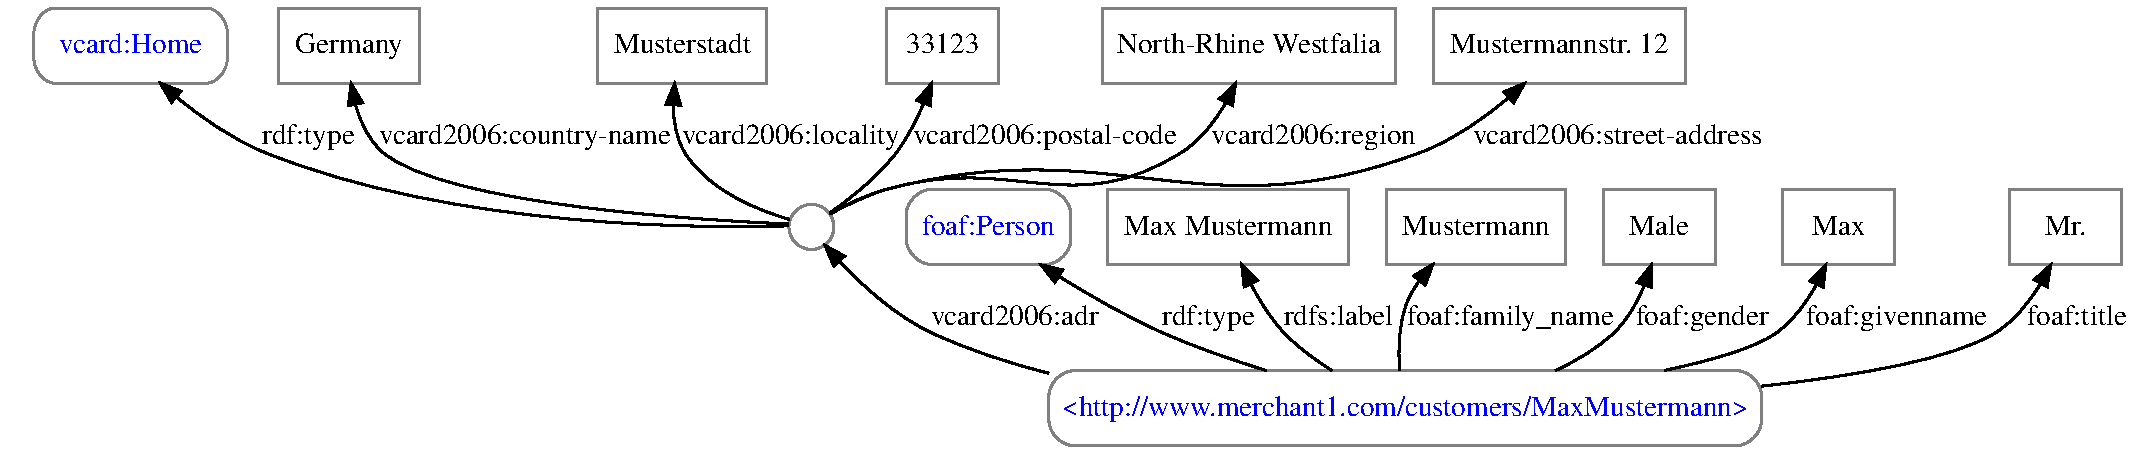
\includegraphics[width=\columnwidth]{images/sample_customer_mustermann.pdf}
	\caption{Graph representation of consumer information from Listing~\ref{lst:sample_customer_mustermann}}
\label{fig:images_sample_customer}
\end{figure}

Still, being able to describe persons and their addresses is just a subset of the entities and relations found in the \gls{E-commerce} scenario. When looking back to the initial \gls{ER} model of an \gls{E-commerce} transaction as shown in Section~\ref{sec:data_model_transactions} one can map the information, which are currently available in the \gls{E-commerce} scenario, to the existing \gls{RDF} vocabularies such as follows (see Table~\ref{tab:map_tx_rdf_vocab}): \@

\begin{table}[H]
\centering
\begin{tabular}{p{5cm}l}
\hline
\textbf{Information} & \textbf{RDF vocabulary} \\
\hline
Consumer & FOAF \\
\hline
Credit Card Owner & FOAF \\
\hline
Billing Address & vCard \\
\hline
Shipping Address & vCard \\
\hline
Location Information & Geo Names \\
\hline
Merchant & GoodRelations \\
\hline
Items & GoodRelations \\
\hline
Item Categories & GoodRelations \\
\hline
Brands & GoodRelations \\
\hline
Payment Types & GoodRelations \\
\hline
\end{tabular}
\caption{Possible usage of \gls{RDF} vocabularies for \gls{E-commerce} transaction information}
\label{tab:map_tx_rdf_vocab}
\end{table}

As this table shows there are some parts of the \gls{E-commerce} \gls{ER} model that can be expressed with existing \gls{RDF} vocabularies extensively --- such as personal related information via \gls{FOAF} and \gls{vCard}, whereas other parts can not be stated in-depth (e.g. credit card information), or are not specified at all (e.g.\ tracking of the delivery). Due to these circumstances one usually have to build an own \gls{RDF} vocabulary or Web ontology that fills in the missing pieces and refers to the existing concepts whenever appropriate.\\

When trying to model the information of a credit card as displayed in Figure~\ref{fig:images_data_model} a possible result will be the \gls{RDFS} specification shown in Listing~\ref{lst:credit_card_vocab}. This definition of a credit card resource explicitly reuses specifications from the \gls{FOAF} and GoodRelations ontologies by specifying that: \@

\begin{itemize}
 \item the owner of a credit card has to be of type ``Person'' from the \gls{FOAF} ontology
 \item the type of a credit card has to be an instance of the type ``PaymentMethodCreditCard'' from the GoodRelations ontology
\end{itemize}

As most of the parts of the \gls{E-commerce} data model shown in Figure~\ref{fig:images_data_model} can not be expressed directly with the existing \gls{RDF} vocabularies, filling in the gaps would mean to come up with a large set of custom entities and relationships.

\begin{listing}[H]
 \inputminted[linenos,
              numbersep=5pt,
              breaklines=true,
              frame=lines]{TURTLE}
              {./samples/vocab_credit_card.ttl}
 \caption{A specification for a credit card in \gls{RDFS}}
\label{lst:credit_card_vocab}
\end{listing}

When analyzing the list of existing and actively used \gls{RDF} vocabularies and ontologies in Table~\ref{tab:used_vocab_rdf}, one will also find the Schema.org schema specification \citep{Schema.org}. This vocabulary was initially designed by the leading search engines (e.g.\ Google, Microsoft and Yahoo!) to allow authors of Web sites to markup their \gls{HTML} documents in a way so that they are better understood by these search engines. The Schema.org vocabulary is actively maintained by its community, includes new concepts with each release, and also offers an extension mechanism to implement additional vocabularies with terms that are not part of the core specifications \citep{SchemaExtensions} yet. In one of the past releases of it the maintainers also introduced all of the existing concepts of the GoodRelation ontology into the Schema.org vocabulary \citep{SchemaGoodRelation}. \\

As the merchants will likely provide semantic meta data for their products and offers to improve their listings on search engine results (also known as \gls{SEO}) using the vocabulary of Schema.org already, one can re-use parts of these information for the \gls{E-commerce} fraud investigation scenario as well. Additionally, the wide-ranging scope of aspects declared in the Schema.org vocabulary can make it a good fit for the collaborative system of the \gls{E-commerce} fraud investigation scenario. When trying to map the initial \gls{ER} model from Section~\ref{sec:data_model_transactions} to the Schema.org core specifications, one will basically come up with a schema as displayed in Figure~\ref{fig:images_schema_org}. \@

\begin{figure}[H]
	\centering
		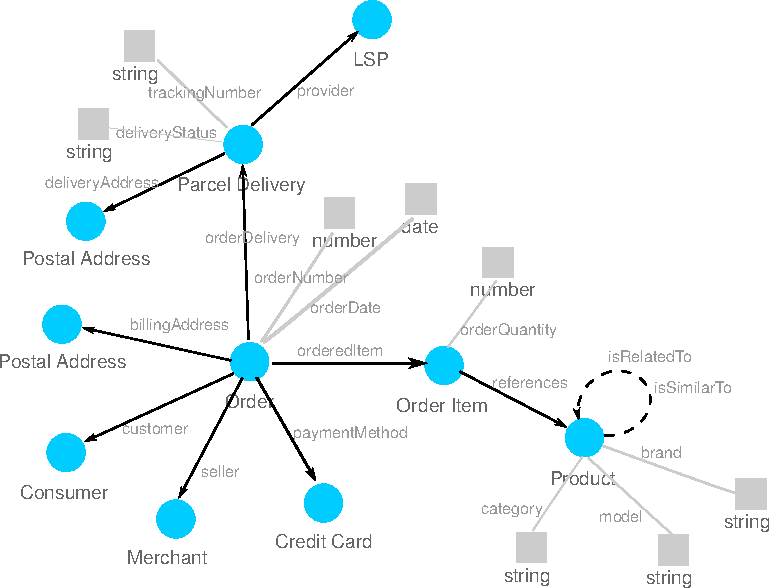
\includegraphics[width=0.8\columnwidth]{images/schema_org_mapping.pdf}
	\caption{Schema.org based mapping of an \gls{E-commerce} transaction}
\label{fig:images_schema_org}
\end{figure}

% subsection reuse_vocab_web (end)

\subsection{Creating a custom vocabulary}
\label{subsec:build_ontology_frauds}

Another possible approach is to define a completely new \gls{RDF} vocabulary or Web ontology for the proposed \gls{E-commerce} fraud investigation system and share that with every possible stakeholder. This specification will define all the entities and relations known to the collaborative system and would describe them in \gls{RDFS} format (see Section~\ref{sec:semantic_web}). \\

A major drawback of this approach is that new partners of the system will have to implement the conversion of their internal data structures to an \gls{RDF} data set, which is compatible with the predefined schema definition, first, before even being able to participate in it. This will limit the general usage of the collaborative system, and will therefore not further considered in detail.

% subsection build ontology (end)

\subsection{Mapping and Linking between vocabularies}

Although it is possible to model an \gls{E-commerce} transaction with the Schema.org specification as shown in Figure~\ref{fig:images_schema_org}, the collaborative system still has to take care of the mapping of the transactional information coming from various sources to be able to combine, analyze and cluster them. As the Semantic Web does not restrict how organizations structure and express their information, and following the ``AAA slogan'', there are likely different \gls{RDF} representations of an \gls{E-commerce} transaction in-use. \\

The \gls{W3C} standards for the Semantic Web also include support for these mapping issues, as they will also come up when trying to combine semantic information available around the Web. Additionally, the Schema.org specification also defines a property, that can be used for that purpose. The following properties are available in the \gls{RDFS}, \gls{OWL} and Schema.org specifications: \@

\begin{itemize}
	\item \textbf{rdfs:label}: a label of a resource in the \gls{RDF} data set can contain a human-friendly name of the resource. These labels are literals of type string and can come with a language specifier in case the resource supports expressions for different languages (see Listing~\ref{lst:rdfs_label_language} for an example).
	\item \textbf{rdfs:seeAlso}: a relation of type seeAlso contains an \gls{URI} to an external resource, that contains additional information for the subject (see Listing~\ref{lst:rdfs_seeAlso_location} for an example).
	\item \textbf{rdfs:isDefinedBy}: the isDefinedBy property is a specialization of the seeAlso relation, in that it specifies a link to the original definition of a resource
	\item \textbf{owl:sameAs, schema:sameAs}: the sameAs relation as specified in the \gls{OWL} and Schema.org vocabularies are providing an unique \gls{URI} that unambiquiously define the subject (see Listing~\ref{lst:schema_sameAs_location} for an example)
\end{itemize}

% subsection map ontology (end)

% sec data_schema (end)
